\documentclass[a4paper, oneside]{memoir}
\usepackage[utf8]{inputenc}
\usepackage[T1]{fontenc}
\usepackage{pifont}
\usepackage{amssymb}
\usepackage{fourier}
\usepackage[dvipsnames]{xcolor}
\usepackage{tikz}
\usepackage{pdfpages}
\usepackage[sfdefault]{roboto}
\usepackage{color}

\tikzstyle{teamshare} = [below, text width=5.4cm, inner sep = 0.5cm, text=white, align=center]
\tikzstyle{cardtext} = [below, text width=5.4cm, inner sep = 0.5cm, text centered]

% Define Commands
\newcommand{\condition}[1]{\textbf{#1}}
\newcommand{\character}[1]{\textbf{#1}}
\newdimen\titlespacing
\titlespacing=0.25cm

% Define Seperators
\newcommand{\redseperator}{\vspace{\titlespacing} \hrulefill {} \ding{100} \hrulefill\\ \vspace{\titlespacing}}
\newcommand{\greenseperator}{\vspace{\titlespacing} \hrulefill {} \bomb{}/\ding{72} \hrulefill\\ \vspace{\titlespacing}}
\newcommand{\greyseperator}{\vspace{\titlespacing} \hrulefill {} \ding{100} \hrulefill\\ \vspace{\titlespacing}}
\newcommand{\purpleseperator}{\vspace{\titlespacing} \hrulefill {} \bomb{}/\ding{72} \hrulefill\\ \vspace{\titlespacing}}
\newcommand{\descriptionseperator}{\vspace{\titlespacing} \hrulefill {} \tiny description \normalsize \hrulefill\\ \vspace{\titlespacing}}
\newcommand{\modifierseperator}{\vspace{\titlespacing} \hrulefill {} \tiny power \normalsize \hrulefill\\ \vspace{\titlespacing}}
\newcommand{\conditionseperator}{\vspace{\titlespacing} \hrulefill {} \tiny condition \normalsize \hrulefill\\ \vspace{\titlespacing}}
\newcommand{\winseperator}{\vspace{\titlespacing} \hrulefill {} \tiny how to win \normalsize \hrulefill\\ \vspace{\titlespacing}}
\newcommand{\redwinsection}{
	\winseperator
	You win if \character{Santa} does not gain the \condition{humbug} condition due to the \character{Grinch} stealing Christmas.
}
\newcommand{\greenwinsection}{
	\winseperator
	\small You win if \character{Santa} gains the \condition{humbug} condition due to the \character{Grinch} stealing Christmas.
}
\setlrmarginsandblock{0.9cm}{*}{1}
\setulmarginsandblock{1.49cm}{*}{1}
\checkandfixthelayout[nearest]
\pagestyle{empty}

\begin{document}
\noindent 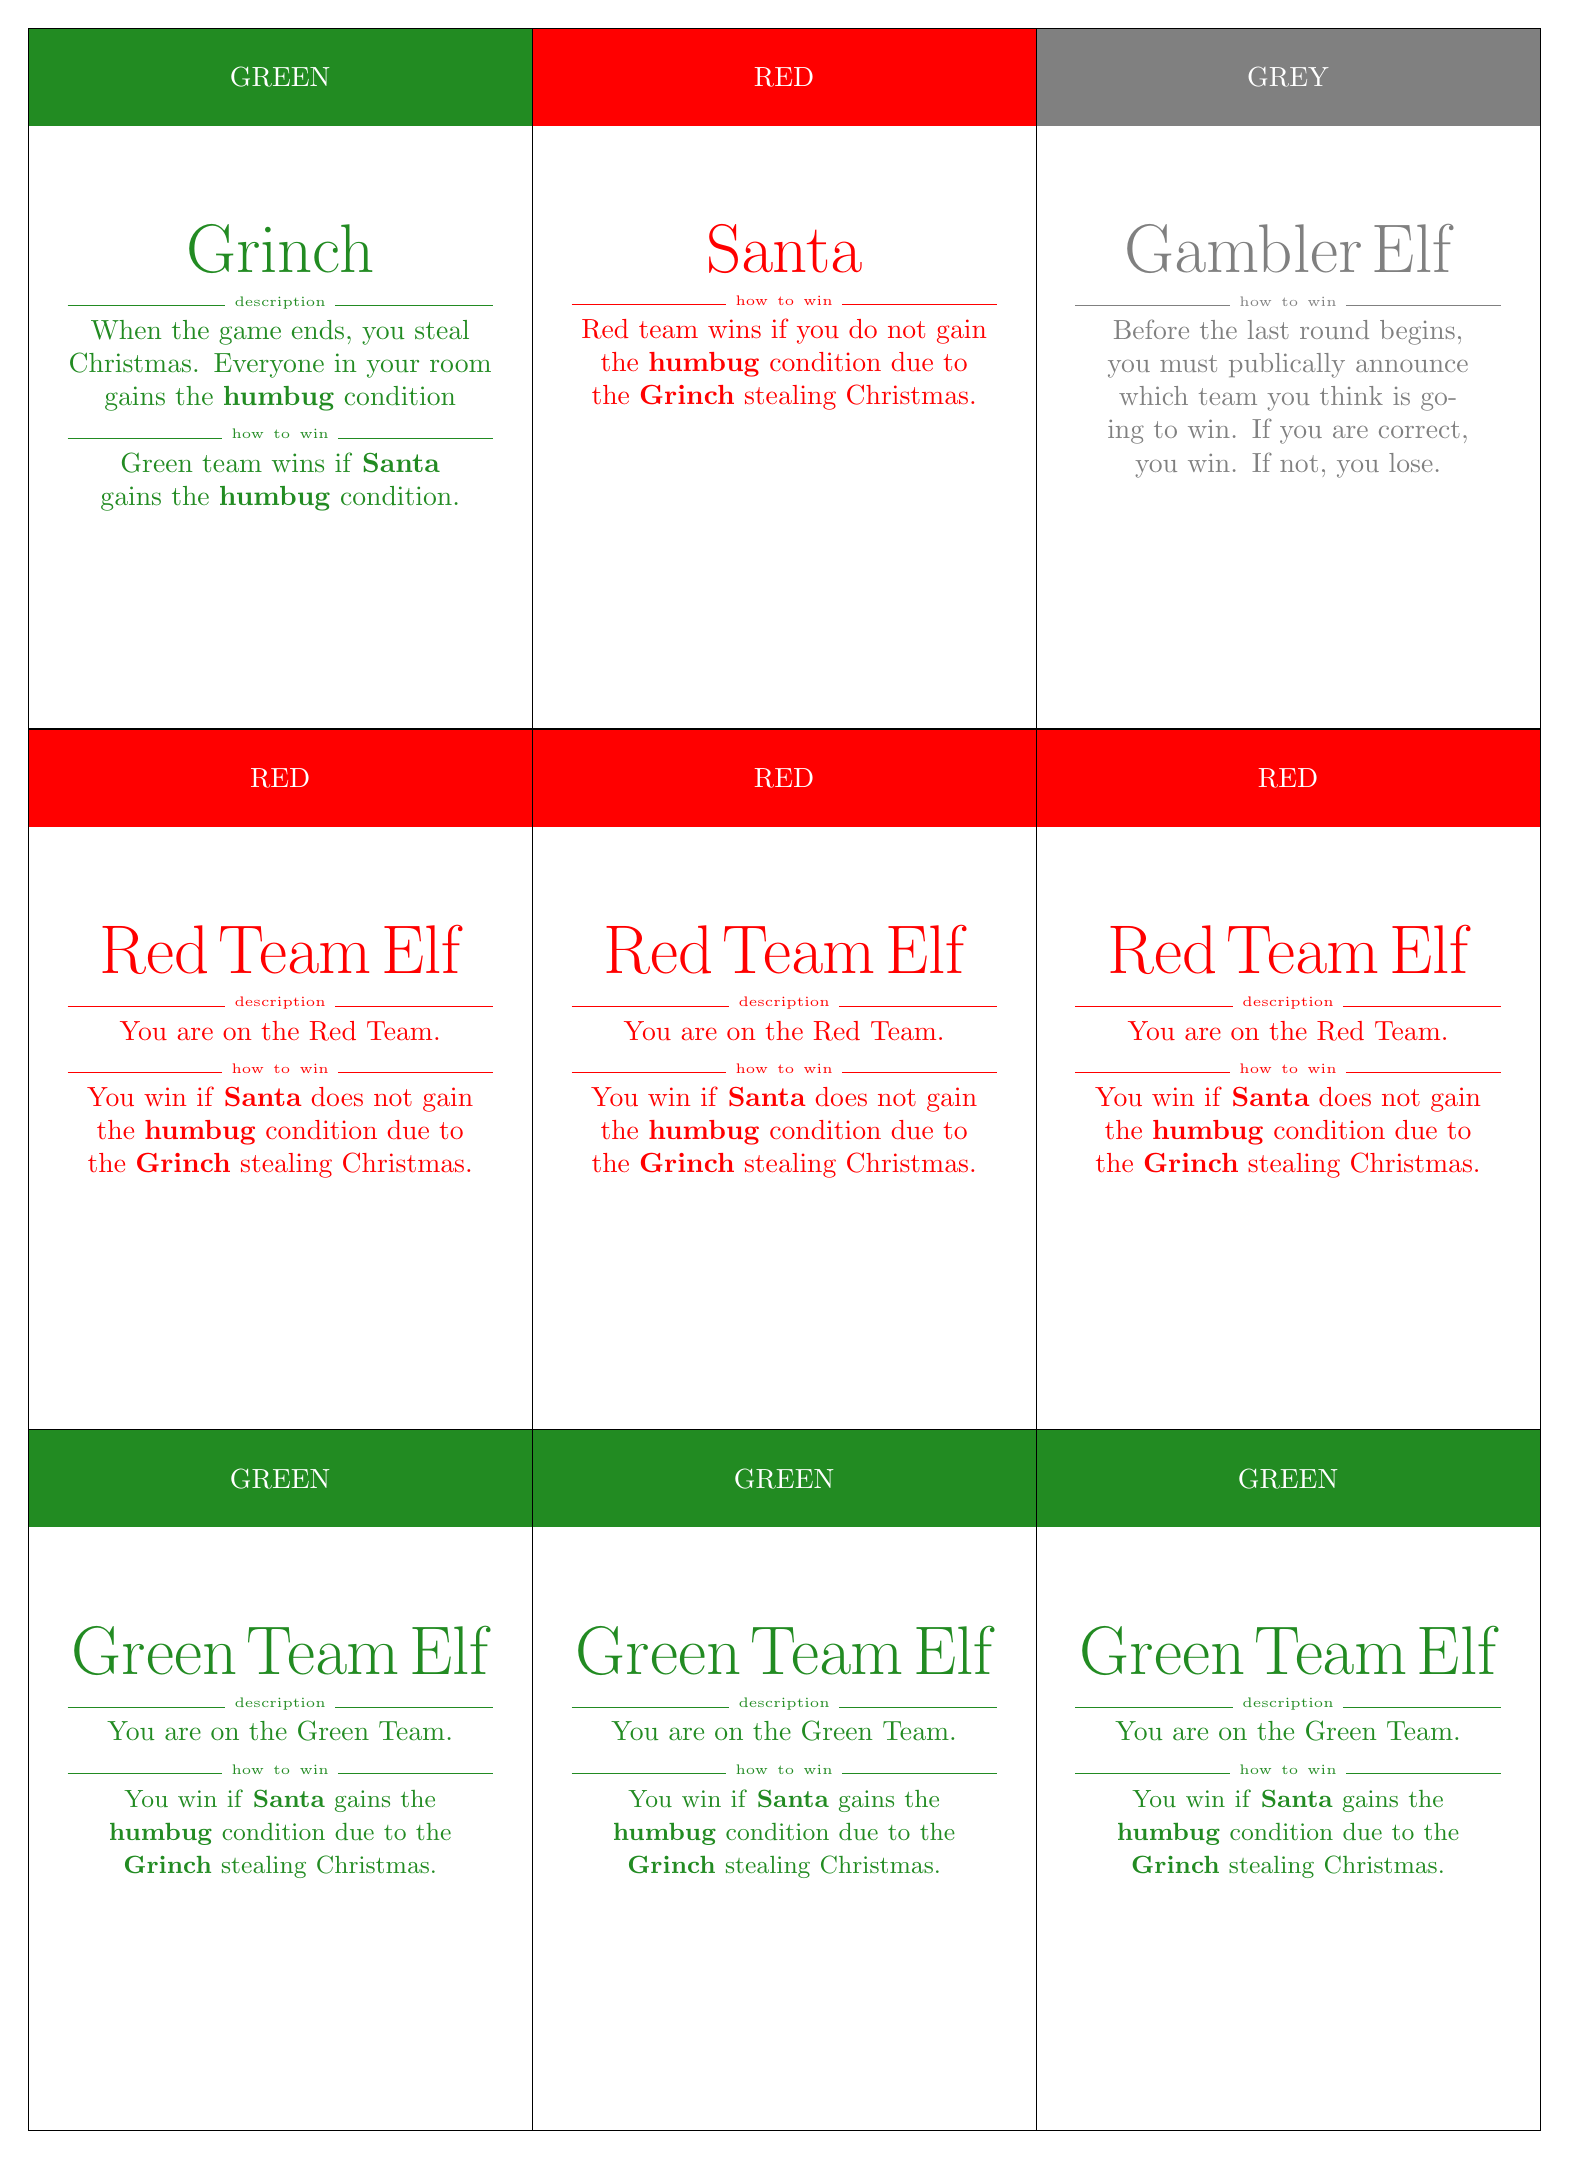
\begin{tikzpicture}[outer sep=0]

% THE GRINCH
\node[teamshare, fill=ForestGreen] (1) at (3.2,26.7) {\HUGE GREEN};
\node[cardtext, text=ForestGreen] at (3.2,24.7) {
	{\Huge Grinch}
	\\\descriptionseperator
	When the game ends, you steal Christmas. Everyone in your room gains the \condition{humbug} condition
	\\\winseperator
	Green team wins if \character{Santa} gains the \condition{humbug} condition.
};

% SANTA
\node[teamshare, fill=red] at (9.6,26.7) {\HUGE RED};
\node[cardtext, text=red] at (9.6,24.7) {
	{\Huge Santa}
	\\\winseperator
	Red team wins if you do not gain the \condition{humbug} condition due to the \character{Grinch} stealing Christmas.
};

% GAMBLER ELF
\node[teamshare, fill=gray] at (16,26.7) {\HUGE GREY};
\node[cardtext, text=gray] at (16,24.7) {
	{\Huge Gambler Elf}
	\\\winseperator
	Before the last round begins, you must publically announce which team you think is going to win. If you are correct, you win. If not, you lose.
};

% RED TEAM ELF
\node[teamshare, fill=red] at (3.2,17.8) {\HUGE RED};
\node[cardtext, text=red] at (3.2,15.8) {
	{\Huge Red Team Elf}
	\\\descriptionseperator
	You are on the Red Team.
	\\\redwinsection
};

% RED TEAM ELF
\node[teamshare, fill=red] at (9.6,17.8) {\HUGE RED};
\node[cardtext, text=red] at (9.6,15.8) {
	{\Huge Red Team Elf}
	\\\descriptionseperator
	You are on the Red Team.
	\\\redwinsection
};

% RED TEAM ELF
\node[teamshare, fill=red] at (16,17.8) {\HUGE RED};
\node[cardtext, text=red] at (16,15.8) {
	{\Huge Red Team Elf}
	\\\descriptionseperator
	You are on the Red Team.
	\\\redwinsection
};

% GREEN TEAM ELF
\node[teamshare, fill=ForestGreen] at (3.2,8.9) {\HUGE GREEN};
\node[cardtext, text=ForestGreen] at (3.2,6.9) {
	{\Huge Green Team Elf}
	\\\descriptionseperator
	You are on the Green Team.
	\\\greenwinsection
};

% GREEN TEAM ELF
\node[teamshare, fill=ForestGreen] at (9.6,8.9) {\HUGE GREEN};
\node[cardtext, text=ForestGreen] at (9.6,6.9) {
	{\Huge Green Team Elf}
	\\\descriptionseperator
	You are on the Green Team.
	\\\greenwinsection
};

% GREEN TEAM ELF
\node[teamshare, fill=ForestGreen] at (16,8.9) {\HUGE GREEN};
\node[cardtext, text=ForestGreen] at (16,6.9) {
	{\Huge Green Team Elf}
	\\\descriptionseperator
	You are on the Green Team.
	\\\greenwinsection
};

\draw (0,0) -- (19.2,0);
\draw (0,8.9) -- (19.2,8.9);
\draw (0,17.8) -- (19.2,17.8);
\draw (0,26.7) -- (19.2,26.7);

\draw (0,0) -- (0,26.7);
\draw (6.4,0) -- (6.4,26.7);
\draw (12.8,0) -- (12.8,26.7);
\draw (19.2,0) -- (19.2,26.7);



\end{tikzpicture}

%Background is not my own. But courtesy of a user on BGG

\includepdf[pages={1}, angle=90]{cardsbackground.pdf}
\pagebreak

\noindent 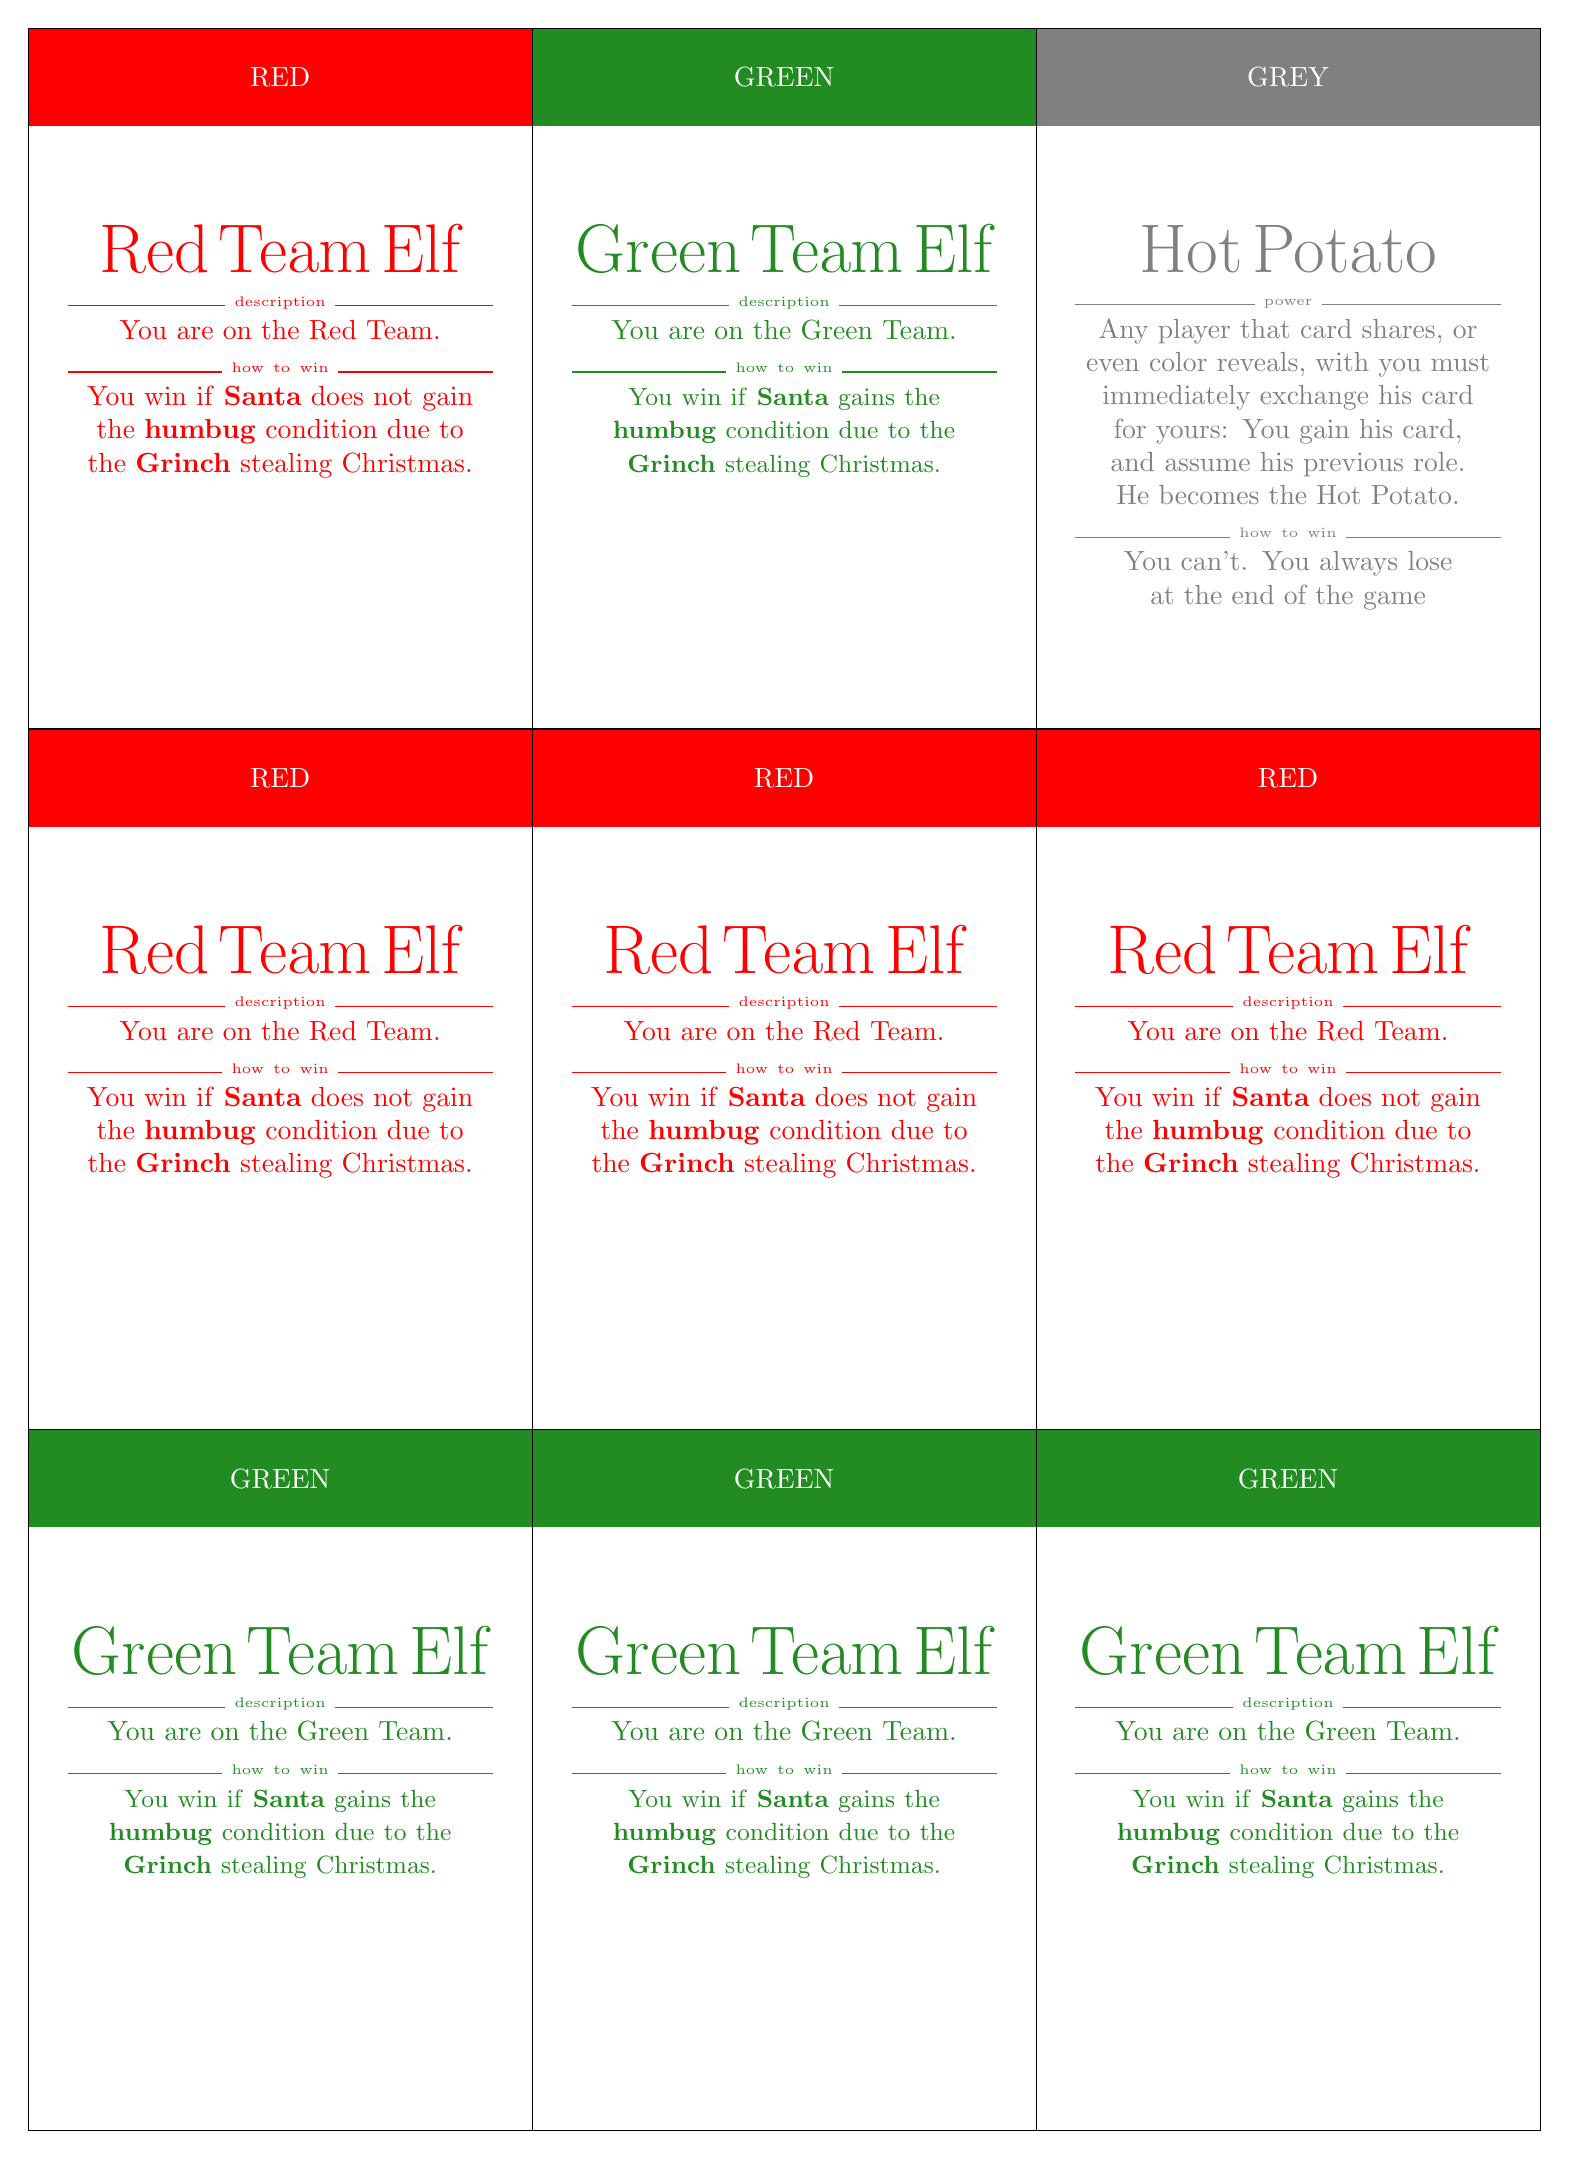
\begin{tikzpicture}[outer sep=0]

% RED TEAM ELF
\node[teamshare, fill=red] (1) at (3.2,26.7) {\HUGE RED};
\node[cardtext, text=red] at (3.2,24.7) {
	{\Huge Red Team Elf}
	\\\descriptionseperator
	You are on the Red Team.
	\\\redwinsection
};

% GREEN TEAM ELF
\node[teamshare, fill=ForestGreen] at (9.6,26.7) {\HUGE GREEN};
\node[cardtext, text=ForestGreen] at (9.6,24.7) {
	{\Huge Green Team Elf}
	\\\descriptionseperator
	You are on the Green Team.
	\\\greenwinsection
};

% HOT POTATO
\node[teamshare, fill=gray] at (16,26.7) {\HUGE GREY};
\node[cardtext, text=gray] at (16,24.7) {
	{\Huge Hot Potato}
	\\\modifierseperator
	Any player that card shares, or even color reveals, with you must immediately exchange his card for yours: You gain his card, and assume his previous role. He becomes the Hot Potato.
	\\\winseperator
	You can't. You always lose at the end of the game	
};

% RED TEAM ELF
\node[teamshare, fill=red] at (3.2,17.8) {\HUGE RED};
\node[cardtext, text=red] at (3.2,15.8) {
	{\Huge Red Team Elf}
	\\\descriptionseperator
	You are on the Red Team.
	\\\redwinsection
};

% RED TEAM ELF
\node[teamshare, fill=red] at (9.6,17.8) {\HUGE RED};
\node[cardtext, text=red] at (9.6,15.8) {
	{\Huge Red Team Elf}
	\\\descriptionseperator
	You are on the Red Team.
	\\\redwinsection
};

% RED TEAM ELF
\node[teamshare, fill=red] at (16,17.8) {\HUGE RED};
\node[cardtext, text=red] at (16,15.8) {
	{\Huge Red Team Elf}
	\\\descriptionseperator
	You are on the Red Team.
	\\\redwinsection
};

% GREEN TEAM ELF
\node[teamshare, fill=ForestGreen] at (3.2,8.9) {\HUGE GREEN};
\node[cardtext, text=ForestGreen] at (3.2,6.9) {
	{\Huge Green Team Elf}
	\\\descriptionseperator
	You are on the Green Team.
	\\\greenwinsection
};

% GREEN TEAM ELF
\node[teamshare, fill=ForestGreen] at (9.6,8.9) {\HUGE GREEN};
\node[cardtext, text=ForestGreen] at (9.6,6.9) {
	{\Huge Green Team Elf}
	\\\descriptionseperator
	You are on the Green Team.
	\\\greenwinsection
};

% GREEN TEAM ELF
\node[teamshare, fill=ForestGreen] at (16,8.9) {\HUGE GREEN};
\node[cardtext, text=ForestGreen] at (16,6.9) {
	{\Huge Green Team Elf}
	\\\descriptionseperator
	You are on the Green Team.
	\\\greenwinsection
};

\draw (0,0) -- (19.2,0);
\draw (0,8.9) -- (19.2,8.9);
\draw (0,17.8) -- (19.2,17.8);
\draw (0,26.7) -- (19.2,26.7);
\draw (0,0) -- (0,26.7);
\draw (6.4,0) -- (6.4,26.7);
\draw (12.8,0) -- (12.8,26.7);
\draw (19.2,0) -- (19.2,26.7);

\end{tikzpicture}


\includepdf[pages={1}, angle=90]{cardsbackground.pdf}

\end{document}